\section{Hello World mit grafischer Benutzeroberfl�che}
\label{ui:helloWorld:section:helloWorldMitGrafischerBenutzeroberfl�che}

Um Tkinter zu initialisieren, muss ein Tk Wurzel-Element erstellt werden.
Dabei handelt es sich um ein gew�hnliches Fenster mit einer Titelleiste und anderer Dekoration,
die vom Betriebssystem bereitgestellt werden.
Generell sollte nur ein Wurzel-Element f�r jedes Programm erstellt werden, das auf h�chster
Ebene vor allen anderen Widget-Elementen steht.

Im folgenden Beispiel wird dazu ein Wurzel-Element mit dem Namen \lstinline$root$ initialisiert.

\lstinputlisting[language=Python]{chapters/userInterface/src/GUI_HelloWorld.py}
\label{ui:helloWorld:lst:lstinputlisting:gui_helloworld}

Damit das Fenster mit Inhalt gef�llt werden kann, m�ssen dem Wurzel-Element weitere
Widgets hinzugef�gt werden. Dazu wurde ein Label mit dem Namen \lstinline$label_1$ angelegt.
Die Parameterliste des \lstinline$Label$-Widgets nimmt als erstes Argument den Namen des Eltern- bzw. Wurzel-Elements und
als zweites Argument den Content bzw. Inhalt des Widgets entgegen.

Als n�chstes ben�tigt Tkinter die Anweisung, wie der Inhalt das Fenster angezeigt werden soll.
Dazu muss eine der Layout-Methoden, in diesem Fall \lstinline$label_1.grid()$, aufgerufen werden.
Das Fenster wird erst sichtbar, sobald die Ereignisschleife \lstinline$mainloop()$ betreten wird.
Anschlie�end kann das Programm wie bereits bekannt ausgef�hrt werden.

\begin{figure}[ht]
	\centering
	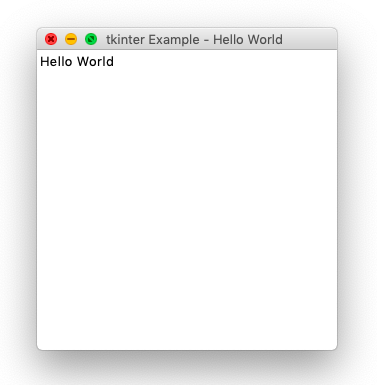
\includegraphics[width=0.8\textwidth]{images/HelloWorldGUI.png}
	\caption{Hello World Beispiel mit grafischer Benutzeroberfl�che}
	\label{ui:helloWorld:img:helloWorldGUI}
\end{figure}

Das Programm wird nun solange ausgef�hrt und bleibt in der Ereignisschleife, bis das Fenster geschlossen wird.
In dieser Schleife werden nicht nur Events wie Nutzereingaben (z.B. Mausklicks oder Tastatureingaben)
verarbeitet, sondern auch die des Fenstersystems (z.B. Redraw-Ereignisse und Fenster-Konfigurationsmeldungen) und
Ereignisse von Tkinter selbst.

\uebung
\aufgabe{UI_aufgabe01}
